%%%%%%%%%%%%%%%%%%%%%%%%%%%%%%%%%%%%%%%%%%%%%%%%%%%%%%%%%%%%%%%%%%%%%
%% This is a (brief) model paper using the achemso class
%% The document class accepts keyval options, which should include
%% the target journal and optionally the manuscript type. 
%%%%%%%%%%%%%%%%%%%%%%%%%%%%%%%%%%%%%%%%%%%%%%%%%%%%%%%%%%%%%%%%%%%%%
\documentclass[journal=jpcafh,manuscript=letter]{achemso}

%%%%%%%%%%%%%%%%%%%%%%%%%%%%%%%%%%%%%%%%%%%%%%%%%%%%%%%%%%%%%%%%%%%%%
%% Place any additional packages needed here.  Only include packages
%% which are essential, to avoid problems later. Do NOT use any
%% packages which require e-TeX (for example etoolbox): the e-TeX
%% extensions are not currently available on the ACS conversion
%% servers.
%%%%%%%%%%%%%%%%%%%%%%%%%%%%%%%%%%%%%%%%%%%%%%%%%%%%%%%%%%%%%%%%%%%%%
\usepackage[version=3]{mhchem} % Formula subscripts using \ce{}

%%%%%%%%%%%%%%%%%%%%%%%%%%%%%%%%%%%%%%%%%%%%%%%%%%%%%%%%%%%%%%%%%%%%%
%% If issues arise when submitting your manuscript, you may want to
%% un-comment the next line.  This provides information on the
%% version of every file you have used.
%%%%%%%%%%%%%%%%%%%%%%%%%%%%%%%%%%%%%%%%%%%%%%%%%%%%%%%%%%%%%%%%%%%%%
%%\listfiles

%%%%%%%%%%%%%%%%%%%%%%%%%%%%%%%%%%%%%%%%%%%%%%%%%%%%%%%%%%%%%%%%%%%%%
%% Place any additional macros here.  Please use \newcommand* where
%% possible, and avoid layout-changing macros (which are not used
%% when typesetting).
%%%%%%%%%%%%%%%%%%%%%%%%%%%%%%%%%%%%%%%%%%%%%%%%%%%%%%%%%%%%%%%%%%%%%
\newcommand*\mycommand[1]{\texttt{\emph{#1}}}

%%%%%%%%%%%%%%%%%%%%%%%%%%%%%%%%%%%%%%%%%%%%%%%%%%%%%%%%%%%%%%%%%%%%%
%% Meta-data block
%% ---------------
%% Each author should be given as a separate \author command.
%%
%% Corresponding authors should have an e-mail given after the author
%% name as an \email command. Phone and fax numbers can be given
%% using \phone and \fax, respectively; this information is optional.
%%
%% The affiliation of authors is given after the authors; each
%% \affiliation command applies to all preceding authors not already
%% assigned an affiliation.
%%
%% The affiliation takes an option argument for the short name.  This
%% will typically be something like "University of Somewhere".
%%
%% The \altaffiliation macro should be used for new address, etc.
%% On the other hand, \alsoaffiliation is used on a per author basis
%% when authors are associated with multiple institutions.
%%%%%%%%%%%%%%%%%%%%%%%%%%%%%%%%%%%%%%%%%%%%%%%%%%%%%%%%%%%%%%%%%%%%%
\author{Maram Susli}
\author{Khidhir Alhameedi}
\author{Dylan Jayatilaka}
\email{dylan.jayatilaka@uwa.edu.au}
\phone{+61 8 64883138}
\affiliation[UWA]
{School of Molecular Sciences, The University of Western Australia, %
35 Stirling Highway, Crawley 6009, Western Australia}

%%%%%%%%%%%%%%%%%%%%%%%%%%%%%%%%%%%%%%%%%%%%%%%%%%%%%%%%%%%%%%%%%%%%%
%% The document title should be given as usual. Some journals require
%% a running title from the author: this should be supplied as an
%% optional argument to \title.
%%%%%%%%%%%%%%%%%%%%%%%%%%%%%%%%%%%%%%%%%%%%%%%%%%%%%%%%%%%%%%%%%%%%%
\title[An \textsf{achemso} demo]
  {Comment on ``Inter/Intramolecular Bonds in \ce{TH5+} (T = C/Si/Ge): 
  \ce{H2} as Tetrel Bond Acceptor and the Uniqueness of Carbon Bonds''}

%%%%%%%%%%%%%%%%%%%%%%%%%%%%%%%%%%%%%%%%%%%%%%%%%%%%%%%%%%%%%%%%%%%%%
%% Some journals require a list of abbreviations or keywords to be
%% supplied. These should be set up here, and will be printed after
%% the title and author information, if needed.
%%%%%%%%%%%%%%%%%%%%%%%%%%%%%%%%%%%%%%%%%%%%%%%%%%%%%%%%%%%%%%%%%%%%%
\abbreviations{RGBI}
\keywords{Tetrel bond, Roby-Gould bond analysis, bond index}

%%%%%%%%%%%%%%%%%%%%%%%%%%%%%%%%%%%%%%%%%%%%%%%%%%%%%%%%%%%%%%%%%%%%%
%% The manuscript does not need to include \maketitle, which is
%% executed automatically.
%%%%%%%%%%%%%%%%%%%%%%%%%%%%%%%%%%%%%%%%%%%%%%%%%%%%%%%%%%%%%%%%%%%%%
\begin{document}

%%%%%%%%%%%%%%%%%%%%%%%%%%%%%%%%%%%%%%%%%%%%%%%%%%%%%%%%%%%%%%%%%%%%%
%% The "tocentry" environment can be used to create an entry for the
%% graphical table of contents. It is given here as some journals
%% require that it is printed as part of the abstract page. It will
%% be automatically moved as appropriate.
%%%%%%%%%%%%%%%%%%%%%%%%%%%%%%%%%%%%%%%%%%%%%%%%%%%%%%%%%%%%%%%%%%%%%
%  \begin{tocentry}
%  
%  Some journals require a graphical entry for the Table of Contents.
%  This should be laid out ``print ready'' so that the sizing of the
%  text is correct.
%  
%  Inside the \texttt{tocentry} environment, the font used is Helvetica
%  8\,pt, as required by \emph{Journal of the American Chemical
%  Society}.
%  
%  The surrounding frame is 9\,cm by 3.5\,cm, which is the maximum
%  permitted for  \emph{Journal of the American Chemical Society}
%  graphical table of content entries. The box will not resize if the
%  content is too big: instead it will overflow the edge of the box.
%  
%  This box and the associated title will always be printed on a
%  separate page at the end of the document.
%  
%  \end{tocentry}

%%%%%%%%%%%%%%%%%%%%%%%%%%%%%%%%%%%%%%%%%%%%%%%%%%%%%%%%%%%%%%%%%%%%%
%% The abstract environment will automatically gobble the contents
%% if an abstract is not used by the target journal.
%%%%%%%%%%%%%%%%%%%%%%%%%%%%%%%%%%%%%%%%%%%%%%%%%%%%%%%%%%%%%%%%%%%%%


%%%%%%%%%%%%%%%%%%%%%%%%%%%%%%%%%%%%%%%%%%%%%%%%%%%%%%%%%%%%%%%%%%%%%
%% Start the main part of the manuscript here.
%%%%%%%%%%%%%%%%%%%%%%%%%%%%%%%%%%%%%%%%%%%%%%%%%%%%%%%%%%%%%%%%%%%%%


Recently, Gnanasekara and Arunan conducted a study on 
the nature of the chemical bonding in the structure of
\ce{TH5+}, (T = C/Si/Ge) using the Atoms in Molecules (AIM)
and Natural Bond Orbital (NBO) methods \cite{Arunan2019}.
They concluded that \ce{SiH5+} and \ce{GeH5+} were both
intermolecular complexes formed between \ce{TH3+} and 
\ce{H2}, stabilised by a 'tetrel bond' (defined
by Bauza {\em et. al.} \cite{Bauza2013}), 
while \ce{CH5+} was pentacoordinate carbon with three 
short and two long C-H covalent bonds and no H-H bond. 

Since the Roby-Gould Bond Index (RGBI) method \cite{Gould2008} 
has recently proved very useful for analysing weakly 
bonded interactions in crystals \cite{Alhameedi2018}, we 
decided to use it to analyse the bonding situation in the 
title compounds. Like the NBO method, the RGBI method is based 
on a one-electron Hilbert-space analysis of the density matrix.
Unlike the NBO method, the RGBI method gives covalent and 
ionic bond indices as expectation values over bond index operators.
A total bond index may be calculated from these two indices
using a Pythagorean rule, and a percentage covalency
or ionicity can be easily obtained from this.
Bond indices may also be obtained between groups of atoms.

We calculated both the bond indices between atoms,
and, between the central atom T and the \ce{H2} moiety
(T-\ce{H2}), as shown in Figure \ref{fig}. Bond indices between \ce{TH3}
and \ce{H2} were also calculated, but were found to be very
similar to the T-\ce{H2} indices, so are not reported.
They were obtained using a B3LYP/6-31G(d) wavefunction,
which we have previously found to be suitable for such 
analyses\cite{Gould2008,Alhameedi2018:IJQC,Alhameedi2018}. 


\begin{figure}
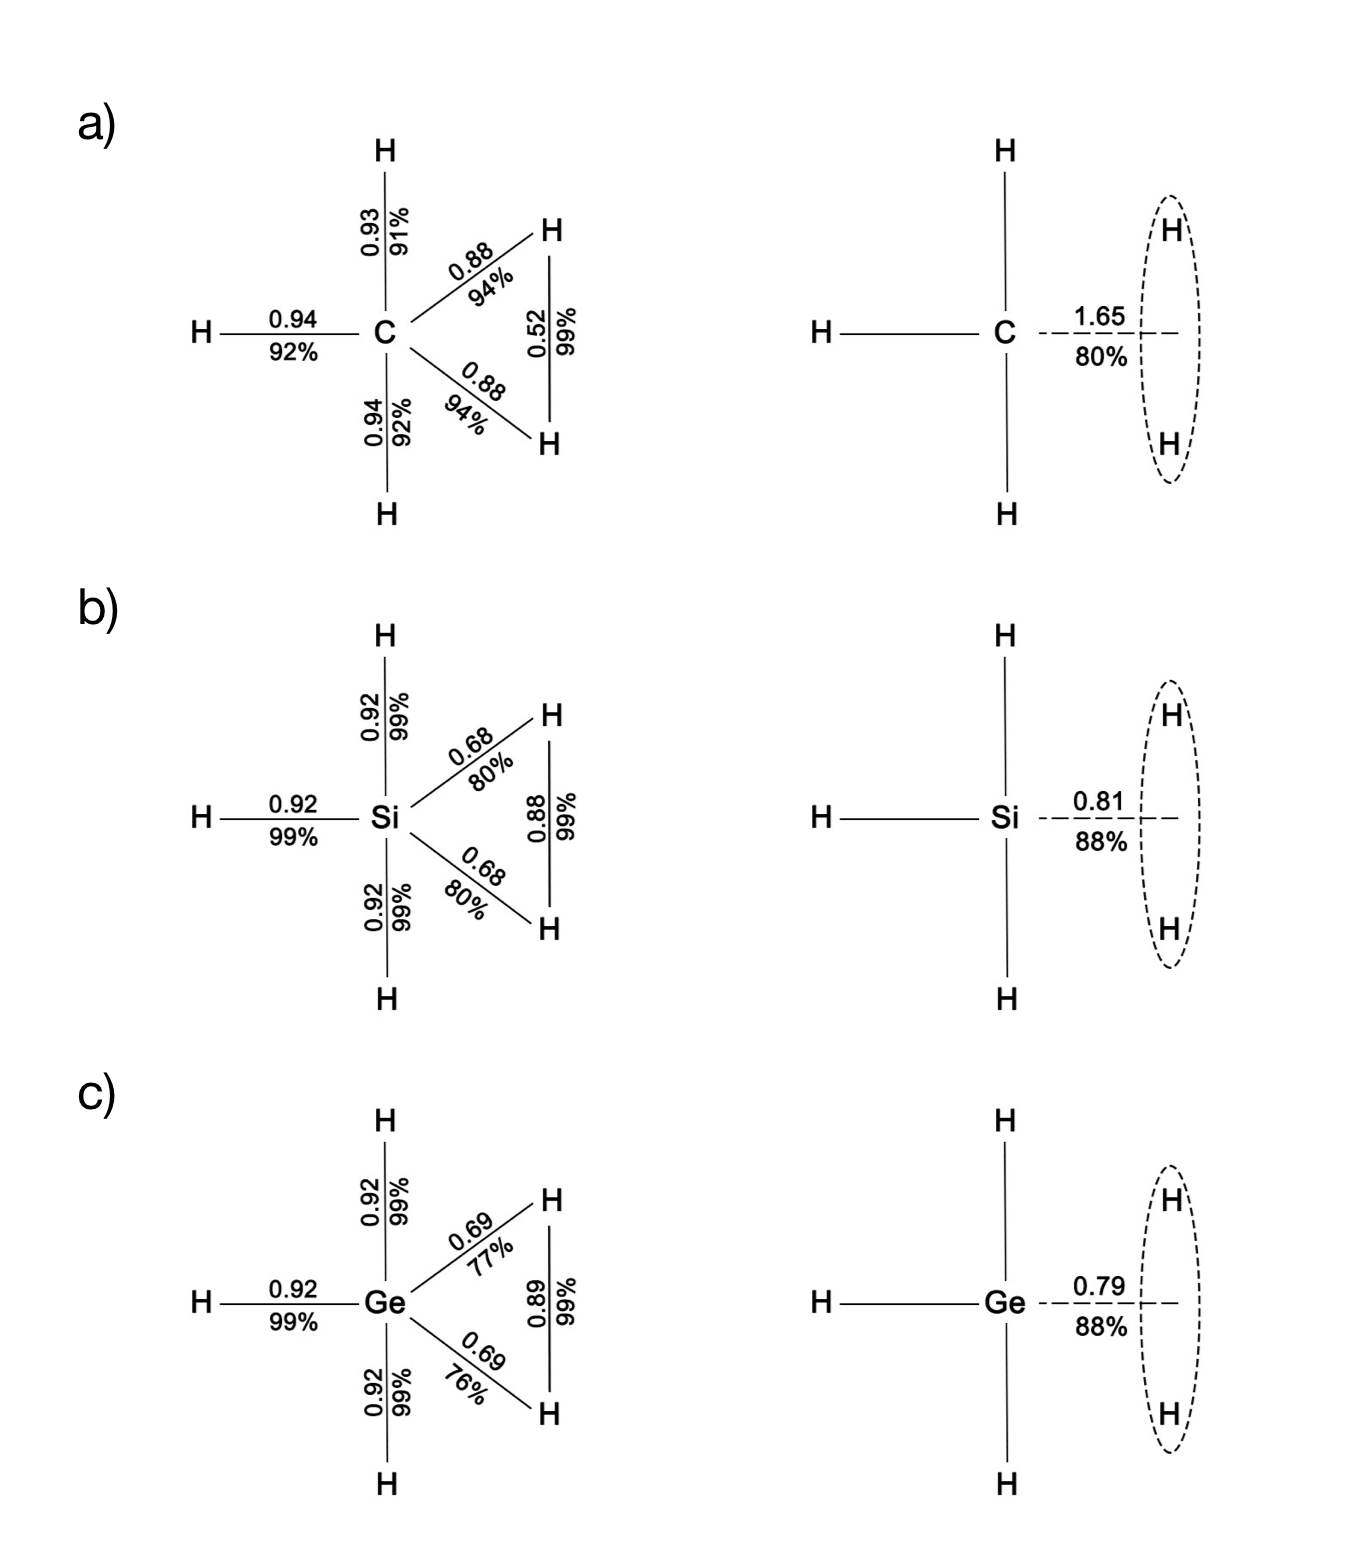
\includegraphics[width=14cm]{TH5allimages.jpg}
\caption{Roby-Gould bond indices and percentage covalency
for bonds between atoms (left) and for the T-\ce{H2} bond (right)
for a) \ce{CH5+}, b) \ce{SiH5+} and c) \ce{GeH5+}.}
\label{fig}
\end{figure}

We shall begin the discussion based on the atom-atom bond indices
in \ce{SiH5+} and \ce{GeH5+}. For these molecules the \ce{H-H} bond index
in the \ce{H2} moiety of these molecules was found to 
be 0.88 and 0.89, respectively. They are covalent, and
slightly smaller in magnitude than the bond index for 
an isolated \ce{H2} molecule, which has a value of 0.98. \cite{Gould2008}
Furthermore, we observe that the bond indices 
for \ce{Ge-H} and \ce{Si-H}, where H is either hydrogen 
in the \ce{H2} moiety, are 0.69 and 0.68, respectively. 
These values are larger than any of the hydrogen-bond 
indices we observed in our previously mentioned study 
of weak interactions in molecular crystals \cite{Alhameedi2018:IJQC}. 
In that work the strongest of the hydrogen bonds was of the 
\ce{OH\bond{...}O} type, with a maximum value of
0.38. Hence, according to the RGBI method, these are 
to be regarded as strong interactions, and not tetrel bonds. 
% DJ: sorry to go over this again, but we say that these
% are larger that the stroingest H-bond, but then we
% say they are *not* tetrel bonds? I am confused.
% They are stronger than H bonds!I think the problem
% is that noewhere have we said what a terel bond is ...
% Didn't we have that before? Where has it gone?
% Now we are like Arunan, who writes a paper on tetrel bonds
% without once clarifying what it is!
This is in contradiction with the conclusions of Gnansekara and 
Arunan, 
% Can we quote the exact statement taht we are in contradiction with?
which were in part based on the long bond lengths for these bonds.

For the interesting case of \ce{CH5+}, the bond index of \ce{H-H} 
in  the \ce{H2} moiety was found to be 0.52. 
This is a half-covalent bond such as would be found in \ce{H2+}. 
Indeed, the Roby-Gould electron population on each H atom in 
the \ce{H2} moiety of \ce{CH5+} is around  ~0.4, which 
corresponds well with the \ce{H2+} view. In contrast, 
by using AIM topological methods, Gnanasekara and Arunan are 
only able to dichotomously classify interactions as either existing 
or not. In this case the authors found no ``bond path'' 
between the H atoms. However, in support of our results
we observe that the ``V'' shaped bond path in \ce{CH5+} 
found by Gnanasekera and Arunan is very similar to the 
``T'' shaped bond path in \ce{SiH5+}, where the top part 
of the ``T'' corresponds to a \ce{H-H} bond. 


For the two \ce{C-H} bonds with H atoms
in the \ce{H2} moiety, the bond indices were found to 
be 0.88. This is only slightly smaller than the
bond index of a \ce{C-H} bond in an isolated \ce{CH4} 
molecule, which has a value of 0.96 \cite{Gould2008}.
Thus, in the RGBI approach, the fact that there 
is a covalent bond between the H atoms in the \ce{H2} 
moiety is not inconsistent with Arunan et al's view that the 
C atom in \ce{CH5+} is pentacoordinate. Indeed, the 
weakening of vicinal bonds via weak interactions with 
other atoms, such as occurs here in \ce{C-H}, has been 
observed by many workers, including by us\cite{Alhameedi2018}, 
and Arunan and coworkers\cite{Shahi2014}. 

We now turn to the case of \ce{TH3+}-\ce{H2} interactions.
Here we obtained a bond index of 1.65 for the \ce{C}-\ce{H2} 
bond in \ce{CH5+}, which is approximately the sum 
of the value of the two single \ce{C-H} bonds of ~0.88. 
This is again inconsistent with the view that the
\ce{CH3-H2+} bond is intermolecular in nature. 
Even in the other \ce{TH5+} compounds, the corresponding bond indices 
are 0.81 and 0.79, respectively---around one covalent 
bond---and certainly not close to the sum of the individual 
bond indices to each H atom in the \ce{H2} moiety. 
All this seems consistent with Arunan et al's view that \ce{CH5+} 
is quite different in nature to the other species. However, 
none of them involves an intermolecular tetrel bond.

In summary, our analysis of the bonding in \ce{TH5+}
reveals that all are pentacoordinate to the central atom,
and all molecules have at least a half-covalent \ce{H-H} 
bond in the \ce{H2} moeity. This is more in line with 
the view that bonding  in \ce{TH5+} molecules is 
``triangular'', as was suggested by Asvany and 
coworkers\cite{Asvany1346} for \ce{CH5+}. 
A deficiency in all these analyses, including our own, 
is that they are done only at the minimum of a highly 
fluctional molecule, so vibrational averaging should 
be taken into account. Nevertheless, we think the 
gradated view of chemical bonding offered by the 
RGBI method is more appropriate to the way chemists
view chemical bonding, rather than the dichotomous 
view offered by the topological methods.















\begin{acknowledgement}

The authors thank Prof. Arunan for bringing his work to our attention, and for providing details of the computations in electronic form.



\end{acknowledgement}

\bibliography{achemso-demo}

\end{document}